% ---------------------------------------------------------------------------
% Task 1 responses. All numbers come from the PA1_PRESET=full run
% (data seed 0, model seed 0, CPU). Tables: results/design/<output>.csv
% Populations: "established" = stations 1-3, "held-out" = station 4.
% Split named in every claim: validation = targets in [9600, 12480).
% ---------------------------------------------------------------------------
\section{Task 1: Forecasting Across Heterogeneous Sensors}

\subsection*{Implementation summary}
\begin{itemize}
  \item \texttt{RawAttentionForecaster.forward}: circular Conv1d embedding of the
        $[B,1,L]$ context, add the learned position table, two encoder blocks, final
        LayerNorm, flatten $[B,L\cdot d]$ and a linear head to $[B,H]$.
  \item \texttt{SeriesDecomposition.forward}: replicate the first and last sample
        $\lfloor m/2\rfloor$ times, \texttt{avg\_pool1d} with stride 1 along time, return
        $(x-T,\,T)$ so that $S+T=x$ exactly.
  \item \texttt{aggregate\_delays}: build the source index $(t-\tau_j)\bmod L$ for every
        example and selected delay, \texttt{gather} the shifted values, weight and sum over
        $j$. Fully vectorised and differentiable in values and weights.
\end{itemize}
All notebook checks pass, including the worked decomposition and delay-aggregation examples.

% ---------------------------------------------------------------------------
\subsection*{Response 1A: expected versus measured ordering (Output 1.1)}

\textbf{Expected ordering, written before Output 1.1.}
Established stations: period-routed ridge $<$ Raw Attention $<$ sensor-specific ridge
$\approx$ shared ridge (RMSE). Held-out station 4: the same, with sensor-specific ridge
unavailable and every model slightly worse than on stations 1--3.

\textbf{Measured (validation, RMSE in m/s$^2$).}

\begin{center}\small
\begin{tabular}{lcccc}
\toprule
Model & Established & Held-out 4 & Params & Fit (s)\\
\midrule
Shared ridge          & 0.767 & 0.876 & 4\,608 & 0.01\\
Sensor-specific ridge & 0.768 & n/a   & 13\,824 & 0.09\\
Period-routed ridge   & \textbf{0.166} & \textbf{0.173} & 59\,904 & 0.03\\
Raw Attention         & 0.426 & 0.607 & 368\,368 & 928\\
\bottomrule
\end{tabular}
\end{center}

\begin{itemize}
  \item \textbf{Ordering held}: routed ridge $<$ Raw Attention $<$ shared $\approx$
        sensor-specific on both populations and in every product.
  \item \textbf{Size of the gaps}: routing cuts shared-ridge RMSE by 78\% on stations
        1--3 (0.767 to 0.166). Raw Attention recovers only about 57\% of that gain
        (0.426) with 6$\times$ the parameters of the routed ridge.
  \item \textbf{Sensor identity adds nothing}: sensor-specific ridge is 0.768 against
        0.767 for shared. Per-product RMSEs match to within 0.01 (A 0.804 vs 0.805,
        C 0.630 vs 0.621). Station identity is not the variable that changes the rule.
  \item \textbf{Across products}: shared ridge is worst on Product B (0.854) and best on
        C (0.621). Routed ridge is flat across products (0.181, 0.164, 0.152).
  \item \textbf{Held-out station}: routed ridge barely moves (0.166 to 0.173, +4\%).
        Raw Attention degrades by 42\% (0.426 to 0.607). A plausible (untested)
        explanation is that its learned mixing partly fits the amplitude, mounting phase
        and drift of the three fitted stations.
  \item \textbf{Revision}: I expected Raw Attention to be closer to the routed ridge.
        The explicit pace variable is worth more than generic context-dependent mixing
        in this world, and it transfers to an unseen sensor because pace is shared by
        the whole line while sensor details are not.
\end{itemize}

% ---------------------------------------------------------------------------
\begin{figure}[h]\centering
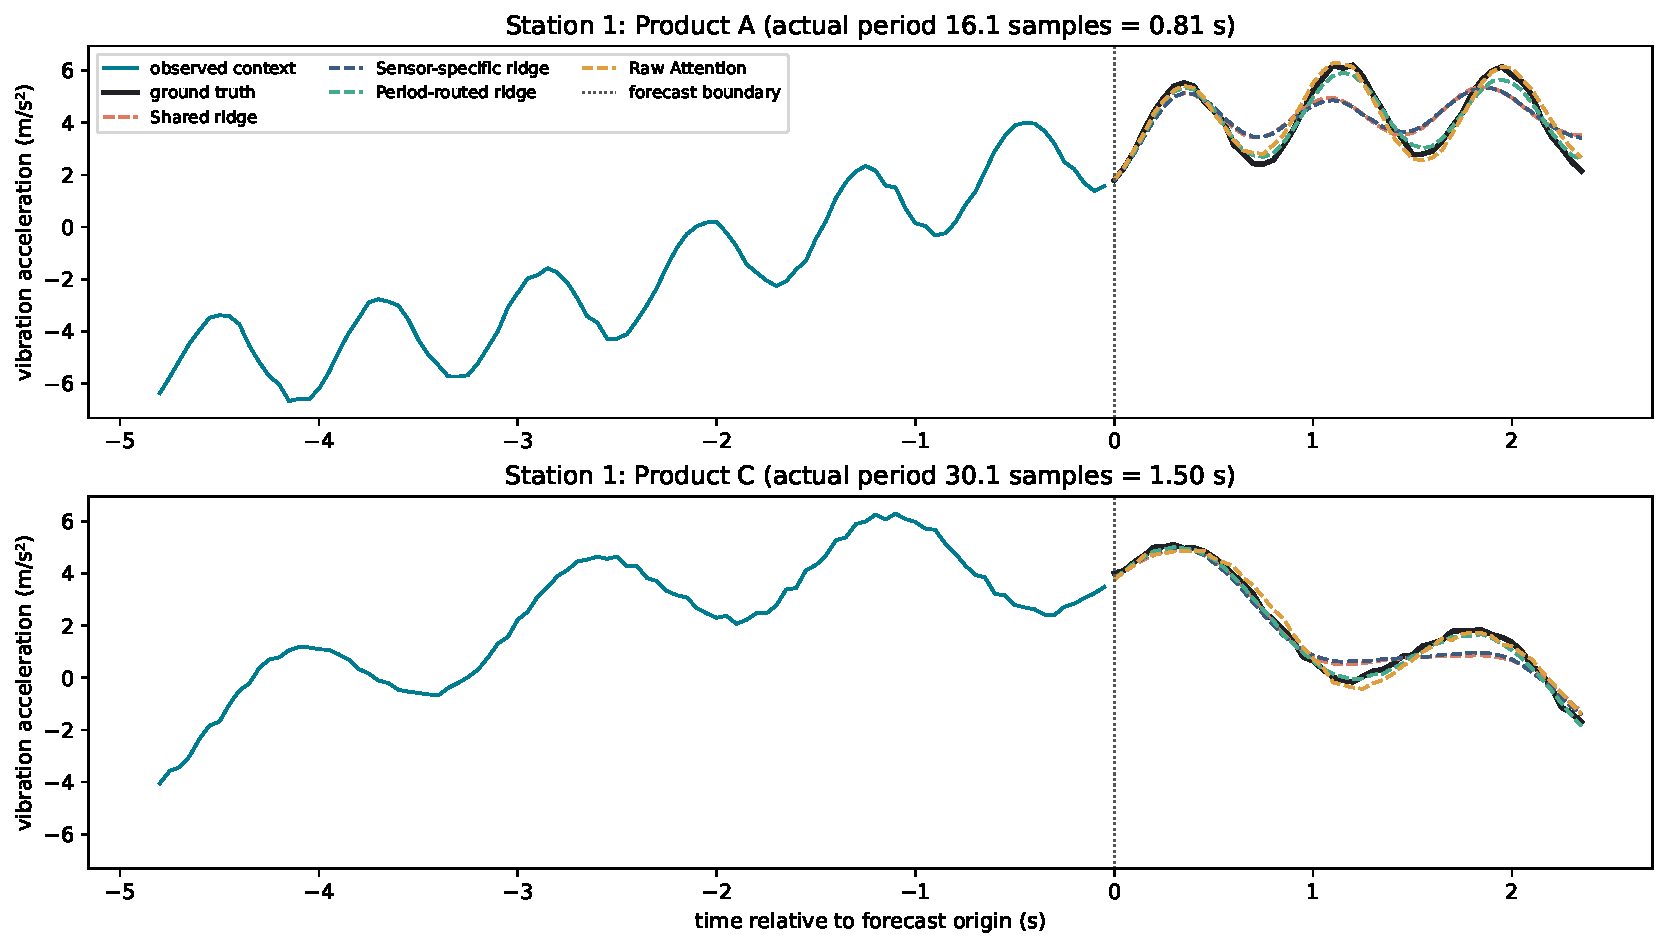
\includegraphics[width=0.49\linewidth]{figures/1.2-1.pdf}\hfill
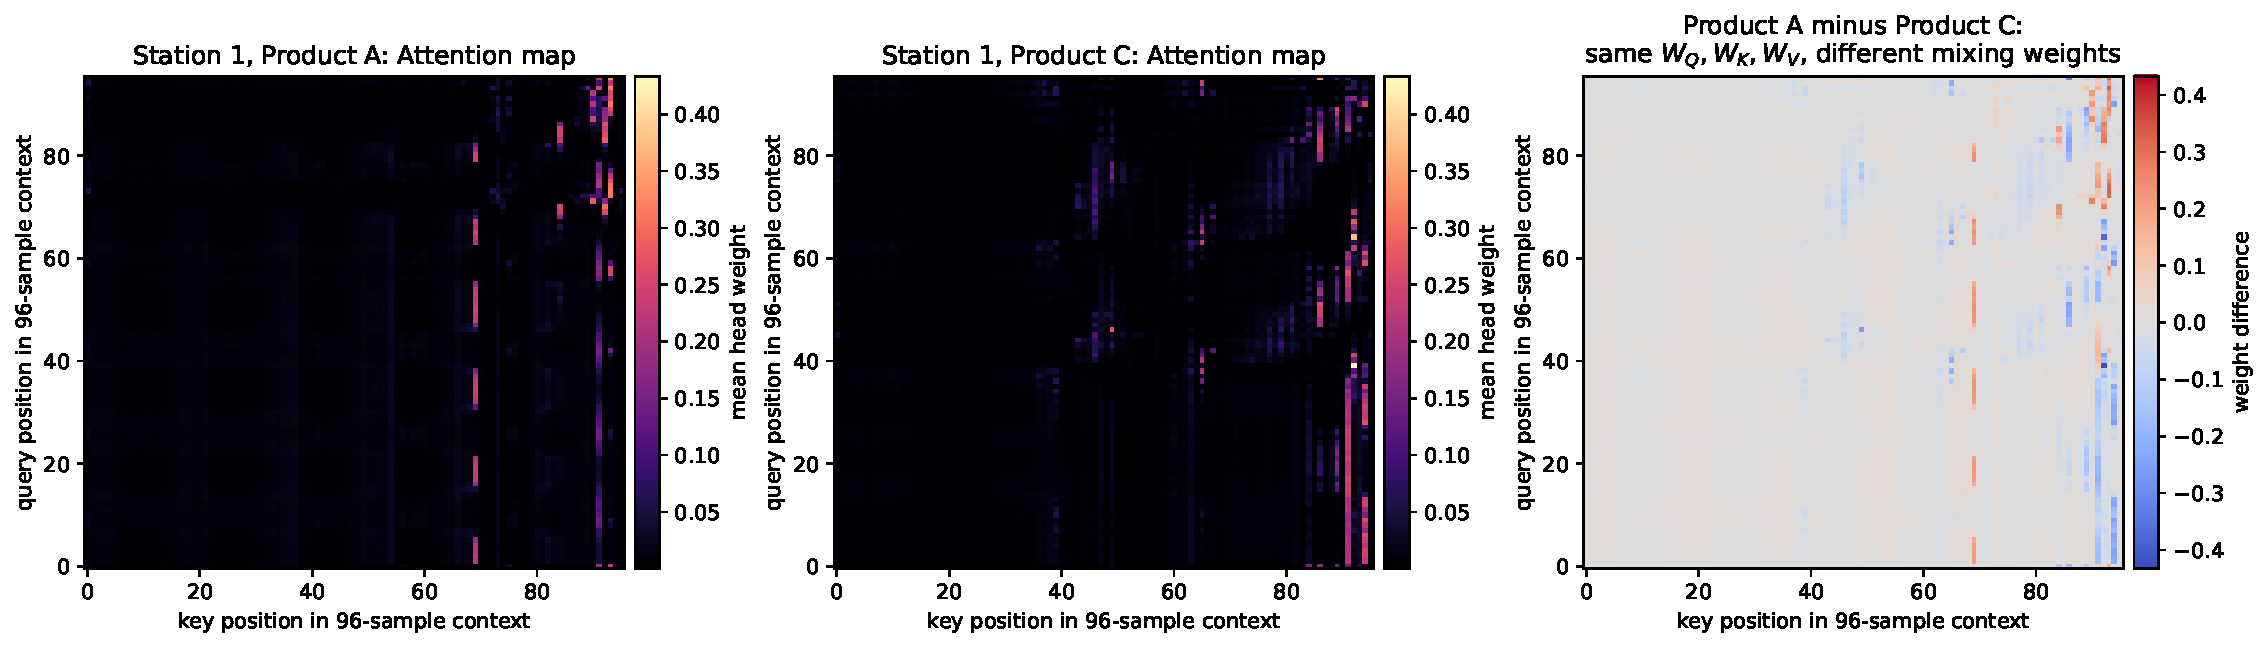
\includegraphics[width=0.49\linewidth]{figures/1.3-1.pdf}
\caption{Output 1.2 (left): station 1 under Products A and C. Output 1.3 (right): Attention maps for the two contexts and their difference.}\label{fig:o12}
\end{figure}

\subsection*{Response 1B: why the rule must depend on context (Outputs 1.2, 1.3)}

\begin{itemize}
  \item \textbf{The compromise in Output 1.2 (validation windows).} On station 1,
        Product A (period 16.1), shared and sensor-specific ridge produce a damped
        oscillation: amplitude is roughly halved and the peaks drift slightly out of phase
        with the truth (window RMSE 0.779 and 0.787). On Product C
        (period 30.1) the same matrix fits much better (0.448 and 0.436).
  \item \textbf{Why.} $\widehat{W}$ in Eq.~(8) is one fixed linear map. Continuing a
        cycle of period 16 and one of period 30 requires different phase advances from
        the same lags. Least squares averages over all training paces. Continuations
        that disagree in phase partly cancel, so the forecast shrinks in amplitude and its
        phase is only approximately right. The damping is the visible cost of averaging
        incompatible continuations.
  \item \textbf{Routed ridge avoids it} because each pace band has its own
        $\widehat{W}$ (0.232 and 0.150 on the same windows). Raw Attention also tracks
        both (0.287 and 0.270) without being told the pace.
  \item \textbf{How Attention changes the operator (Output 1.3, validation windows).} $W_Q, W_K, W_V$ are
        the same for both windows. The weights $\mathrm{softmax}(QK^\top/\sqrt{d_h})$
        are recomputed from each window, so the mixing matrix differs: mean absolute
        difference 0.011 per entry but up to 0.433 on individual query and key pairs.
        The Product A map concentrates on a few key columns late in the context, the
        Product C map spreads over bands near positions 40 to 95.
  \item \textbf{Contrast.} Ridge applies $\hat z = x^\top\widehat{W}$ with the same
        $\widehat{W}$ for every context. Attention applies $\hat z = f(A(x)\,V(x))$ where
        $A(x)$ is built from the input. Output 1.3 shows only that the mixing depends on
        the context, not that it has recovered the physical period.
\end{itemize}

% ---------------------------------------------------------------------------
\subsection*{Response 2: separating slow structure from repetition (Outputs 2.1--2.3)}

\begin{itemize}
  \item \textbf{Selected width: $m=41$}, chosen by the harness on training windows of
        stations 1--3 via the oracle recovery score (Output 2.2: raw 0.687, widths
        17/25/33/41 give 0.980, 0.989, 0.993, 0.998).
  \item \textbf{Visual change (Output 2.1, validation window, station 2, Product C,
        period 32).} Width 17
        leaves the trend bending with each vibration cycle and the residual has uneven
        peaks. As $m$ grows the trend becomes a smooth S-shaped ramp and the residual
        becomes a clean, centred oscillation (residual std grows from 0.58 to 1.57
        m/s$^2$ because less of the cycle is absorbed into $T$). The period projection
        score has a clear (broad) peak near 32 after decomposition and is nearly flat on
        the raw context.
        Edge windows are slightly biased because of endpoint replication.
  \item \textbf{Empirical change (Output 2.3, validation).} Attention + decomposition
        vs Raw Attention: established RMSE 0.426 to 0.297 ($-30\%$, MSE 0.182 to 0.088),
        held-out 0.607 to 0.441 ($-27\%$). Every product improves on both populations,
        for example held-out Product A 0.616 to 0.368. Parameters rise only from 368\,368 to
        373\,024.
  \item \textbf{Why a moving average fits this world.} The drift has a 240-sample scale,
        6--17 times longer than the 14--36-sample vibration. A centred box filter of
        width $m$ removes a sinusoid of period $P$ exactly when $m$ is a multiple of
        $P$ and attenuates it strongly when $m>P$, while passing a slow ramp almost
        unchanged. The 41-sample window is longer than every pace yet much shorter than
        the drift scale, so it separates the two by time scale.
  \item \textbf{Why the oracle diagnostic is a sound selector.} It uses training
        windows only and a quantity (the true period) that exists only in simulation to
        score whether $S$ exposes the repetition. It is not an input to any forecaster,
        so it selects the filter without touching validation or test data.
  \item \textbf{Where it fails / alternative.} If the drift contained a step change or
        a curvature on the same time scale as the vibration (e.g.\ a load jump
        mid-context), the box filter would smear the step into both streams. STL or a
        local-polynomial (LOESS) trend assumes a smooth but locally curved trend and
        fits edges with one-sided polynomials, and a learnable (trainable-kernel)
        decomposition assumes the separation itself should be learned from data.
\end{itemize}

% ---------------------------------------------------------------------------
\begin{figure}[h]\centering
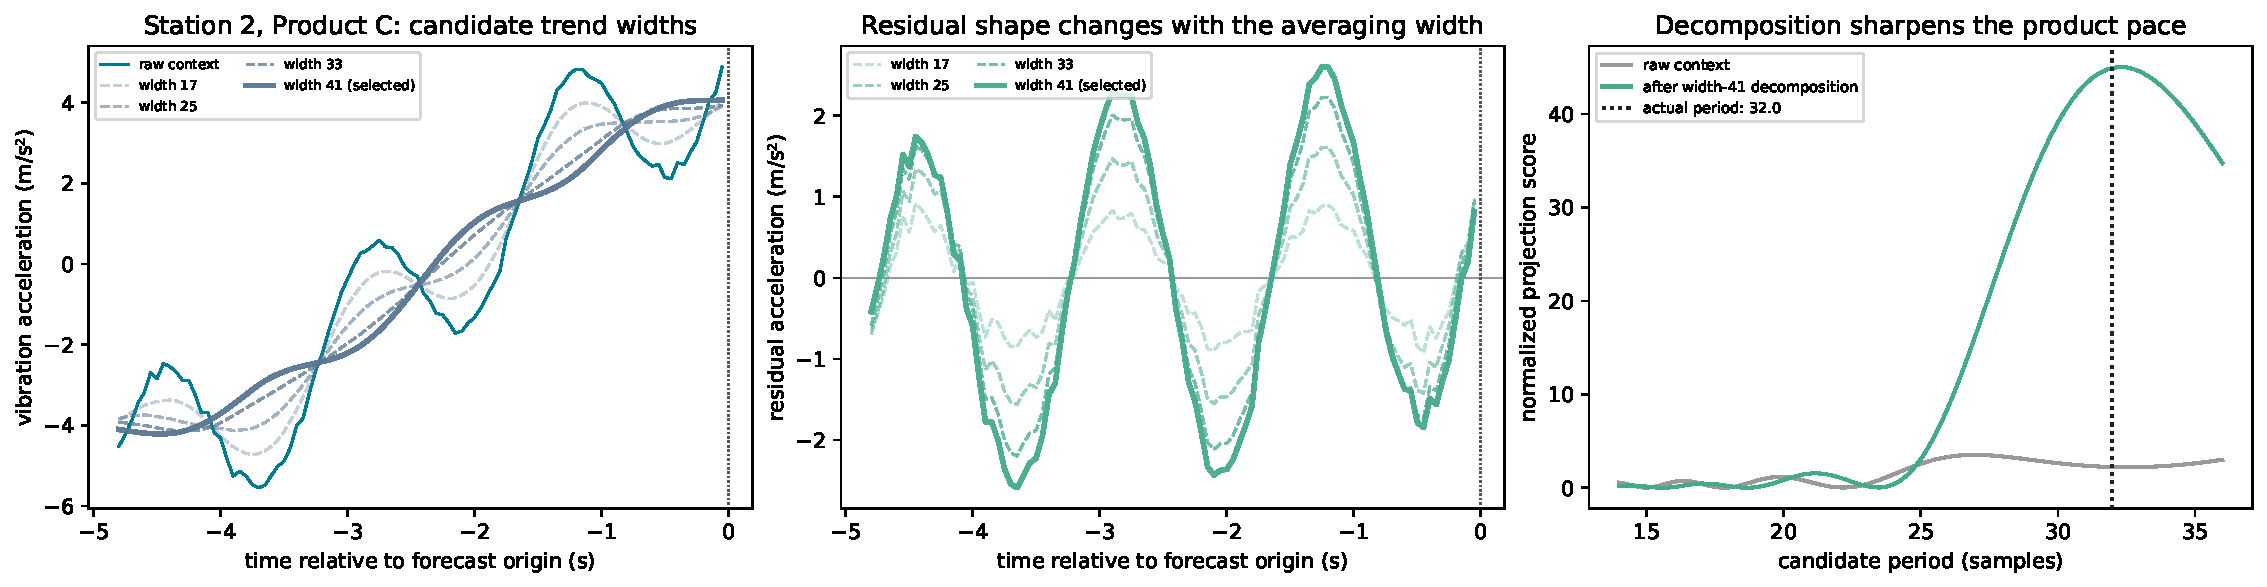
\includegraphics[width=0.95\linewidth]{figures/2.1-1.pdf}
\caption{Output 2.1: candidate trend widths, residuals and the period projection before and after width-41 decomposition.}\label{fig:o21}
\end{figure}

\subsection*{Response 3: mixing by temporal delay (Outputs 3.1, 3.2)}

\begin{itemize}
  \item \textbf{Checks.} Output 3.1 reproduces the direct circular correlation
        $[4,-4,4,-4]$ for $[1,3,1,3]$. The worked aggregation gives
        $z_0=\tfrac34 v_3+\tfrac14 v_1=35$, confirming position $t$ reads $t-\tau$.
  \item \textbf{Strongest recurrence (Output 3.2, validation window).} For station 2,
        Product A (actual period $P=16.13$), the residual correlation peaks at lags 16 and
        32, i.e.\ $P$ and $2P$ rounded to integers, with correlations 0.896 and 0.897, and
        again near 48 ($3P$, about 0.89). The troughs near 8, 24 and 40 are the
        half-period anti-alignments. Integer multiples appear because a shift by $kP$ also
        aligns peaks with peaks.
  \item \textbf{Why decomposition cleans the evidence.} On the raw context the curve
        falls from about 0.45 at lag 8 to about $-0.55$ near lag 40, with only a small
        plateau around lags 26 to 32 and no peak at 16 or 32. A rising ramp stays similar to itself after small shifts
        and dissimilar after large circular shifts (the wrap puts the high end next to
        the low end), so the drift dominates every lag. Removing $T$ leaves the
        oscillation, and lags that are multiples of $P$ then stand out by about 0.9. The
        delay mixer ranks delays by exactly this kind of score (on learned $q,k$), so it
        can only choose good delays if the slow part does not swamp the ranking.
  \item \textbf{Consequence in the models (Output 4.1).} The delay mixer alone gives the
        largest single gain (established RMSE 0.426 to 0.219) and delay + decomposition
        is best among neural models (0.199), consistent with this diagnostic.
  \item \textbf{Where the bias is wrong.} An isolated transient, such as a bearing knock
        or a jam that appears once in the context, has no recurrence. Circular delay
        scores spread its energy over many lags, top-$K$ selection then copies shifted
        versions of the transient into positions where it never happened, and the
        forecast either echoes a spurious repeat or averages it away. The same happens
        when the period drifts within the context, because no single delay aligns the
        early and late cycles.
\end{itemize}

% ---------------------------------------------------------------------------
\begin{figure}[h]\centering
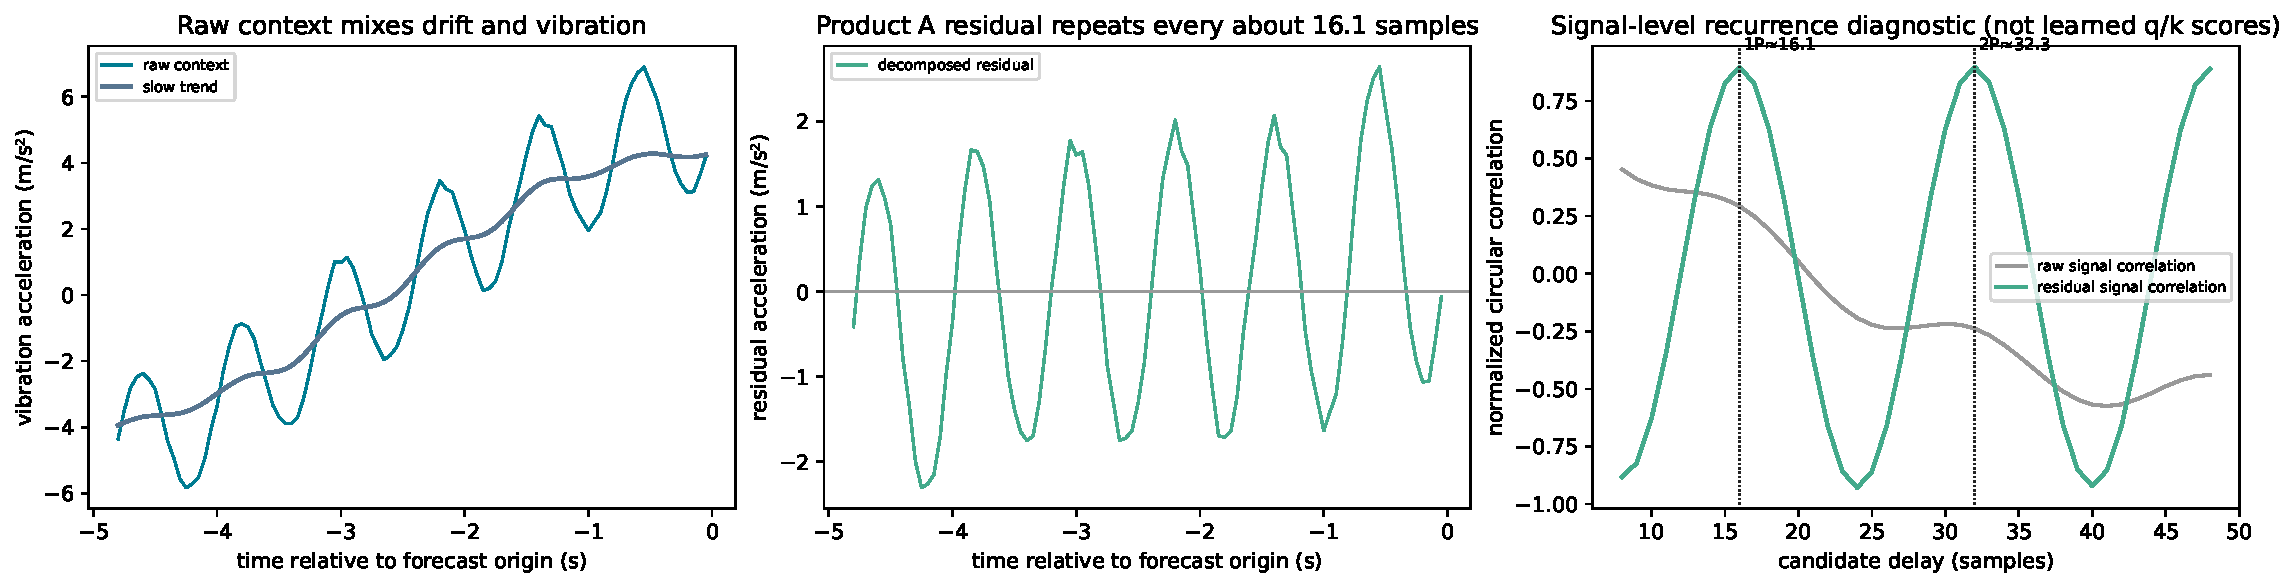
\includegraphics[width=0.95\linewidth]{figures/3.2-1.pdf}
\caption{Output 3.2: signal-level recurrence diagnostic (raw vs decomposed residual correlation), not learned q/k scores.}\label{fig:o32}
\end{figure}

\subsection*{Response 4: compare designs and deploy (Outputs 4.1--4.3)}

\textbf{(a) Prediction, written before Output 4.1.}
Decomposition should help most when the slow component is prominent, because it
removes the ramp before the mixer sees it and gives the trend its own linear head. The
delay mixer on raw input would rank delays by the ramp's self-similarity instead of the
vibration.

\textbf{(b) Validation errors, established stations (MSE in (m/s$^2$)$^2$).}

\begin{center}\small
\begin{tabular}{lccccr}
\toprule
Model & RMSE & MSE & Held-out RMSE & Held-out MSE & Params\\
\midrule
Shared ridge              & 0.767 & 0.588 & 0.876 & 0.767 & 4\,608\\
Sensor-specific ridge     & 0.768 & 0.590 & n/a   & n/a   & 13\,824\\
Period-routed ridge       & \textbf{0.166} & \textbf{0.028} & \textbf{0.173} & \textbf{0.030} & 59\,904\\
Raw Attention             & 0.426 & 0.182 & 0.607 & 0.369 & 368\,368\\
Raw delay mixer           & 0.219 & 0.048 & 0.342 & 0.117 & 368\,370\\
Attention + decomposition & 0.297 & 0.088 & 0.441 & 0.195 & 373\,024\\
Autoformer-inspired       & 0.199 & 0.039 & 0.239 & 0.057 & 373\,026\\
\bottomrule
\end{tabular}
\end{center}

% Interpretation below is limited to 200 words.
\textbf{Interpretation.} Both switches help on their own. On stations 1--3 (validation
MSE), decomposition lowers Raw Attention by 0.094 and delay mixing by 0.134. The
combined model gains 0.142, less than their sum (0.227), so the gains overlap rather
than stack. This is consistent with both switches exploiting the same drift-plus-cycle
structure, although the 2$\times$2 design cannot identify the cause. Station 4 shows
the same pattern (gains 0.174 and 0.252 alone, 0.311 combined). The switches are not
uniformly additive per window either: in Output 4.1's contrasting cases the combined
model cuts a station-4 Product B window from 1.386 to 0.189 but loses on a station-2
Product A window (0.353 vs 0.139 for the raw delay mixer). Along the horizon (Output
4.2, validation, stations 1--3), every model starts near 0.11--0.15 m/s$^2$ at step 1
and diverges afterwards. Raw Attention grows 3.5$\times$ by step 48 (0.151 to 0.525),
the Autoformer-inspired model only 1.7$\times$ (0.136 to 0.235). On station 4 the raw delay
mixer degrades sharply late in the horizon (0.635 at step 48), whereas the combined
model stays near 0.30 (station 4).

\textbf{(c) Deployment.} Period-routed ridge for \textbf{both} populations. It has the
lowest validation RMSE on stations 1--3 (0.166 vs 0.199 for the best neural model) and
on station 4 (0.173 vs 0.239), about 6$\times$ fewer parameters and a closed-form fit
in under 0.1 s instead of 1\,424 s. It needs no station identity, so it transfers to
station 4. Test results (Output 4.3) confirm the choice without being used for it:
0.161 on stations 1--3 and 0.183 on station 4.

\begin{figure}[h]\centering
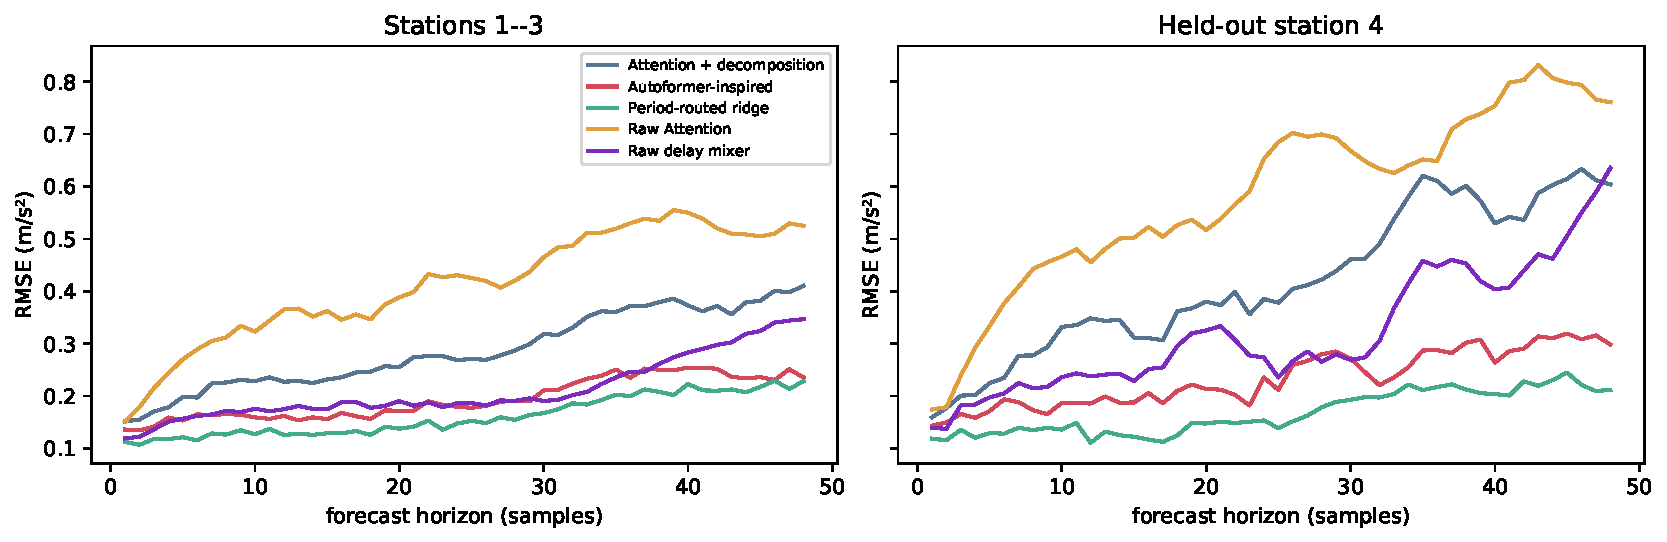
\includegraphics[width=0.95\linewidth]{figures/4.2-1.pdf}
\caption{Output 4.2: validation RMSE along the 48-step horizon, stations 1--3 (left) and station 4 (right).}\label{fig:o42}
\end{figure}
